\documentclass[10pt,aspectratio=169]{beamer}

\usepackage{../../common/foundationsmacro-beamer}
\usepackage[english]{babel}
\usepackage{amsmath}
\usepackage{amssymb}
\usepackage{graphicx}
\usepackage{booktabs}
\usepackage[compatibility=false]{caption}
\usepackage{tikz}

\usetikzlibrary{positioning}
\setbeamertemplate{caption}[numbered]

\title[GDP Accounting]{Chapter 1: Gross Domestic Product}
\author[Bueren]{Jes\'{u}s Bueren}
\institute{Cat\'{o}lica-Lisbon}
\date{2026--2027}



\begin{document}
\begin{frame}[plain]
    \titlepage
\end{frame}

\section{GDP}
\subsection{GDP Accounting}
\begin{frame}{GDP Accounting}
\begin{itemize}
\item One of the basic questions economists are interested in, when analyzing a country, is how much is produced in that country in a given year
\itemvso The basic measure of this is a country's gross domestic product (GDP)
\itemvso The idea is simple: to record the value of everything that is produced in the country in a year and add it up
\itemvso GDP accounts can be constructed in three different (but equivalent) ways, based on measuring:
\begin{enumerate}
\itemvso production
\itemvso income
\itemvso expenditures
\end{enumerate} 
\end{itemize}
\end{frame}

\begin{frame}{US GDP in 2017}
\begin{table}[ht!]
\centering
\captionsetup{labelformat=empty}
\caption{\small Table: US GDP in 2017 according to the three methods (billions of dollars). Source: BEA.}
\resizebox{0.9\linewidth}{!}{%
\begin{tabular}{l r l r l r}
\toprule
\multicolumn{2}{c}{\textbf{Production}} & 
\multicolumn{2}{c}{\textbf{Income}} & 
\multicolumn{2}{c}{\textbf{Expenditure}} \\
\midrule
Agriculture           & 169   & Employee Compensation & 10,421 & Consumption    & 13,321 \\
Mining                & 269   & Corporate Profits      & 1,807  & Investment     & 3,368 \\
Utilities             & 308   & Proprietors’ Income    & 1,501  & Gov. Spending  & 3,374 \\
Construction          & 781   & Rental Income          & 730    & Exports        & 2,350 \\
Manufacturing         & 2,180 & Depreciation           & 3,116  & Imports        & -2,929 \\
Wholesale \& Retail   & 2,261 & Interest Income        & 768    &                &        \\
Transportation        & 609   & Taxes                  & 1,286  &                &        \\
Media                 & 1,051 & Statistical Discrep.   & -143   &                &        \\
Finance \& Insurance  & 1,466 &                        &        &                &        \\
Real Estate           & 2,591 &                        &        &                &        \\
Professional Services & 2,426 &                        &        &                &        \\
Education \& Health   & 1,700 &                        &        &                &        \\
Arts \& Entertainment & 805   &                        &        &                &        \\
Other Services        & 416   &                        &        &                &        \\
Government            & 2,454 &                        &        &                &        \\
\midrule
\textbf{Total}        & \textbf{19,485} & \textbf{Total} & \textbf{19,485} & \textbf{Total} & \textbf{19,485} \\
\bottomrule
\end{tabular}%
}
\end{table}
\end{frame}

\begin{frame}{GDP Accounting}

\begin{itemize}
\item GDP can be measured in three equivalent ways:
\begin{itemize}
    \item production \hspace{1em} \item income \hspace{1em} \item expenditure
\end{itemize}

\medskip

\item Using the expenditure approach, GDP is given by:
\[
Y = C + I + G + X - M
\]
\end{itemize}
\vspace{-0.3cm}
\begin{columns}[T]
\begin{column}{0.48\textwidth}
\begin{itemize}
\item[-] \(Y\): Gross Domestic Product
\item[-] \(C\): Private consumption
\item[-] \(I\): Investment
\end{itemize}
\end{column}

\begin{column}{0.48\textwidth}
\begin{itemize}
\item[-] \(G\): Government purchases
\item[-] \(X\): Exports
\item[-] \(M\): Imports
\end{itemize}
\end{column}
\end{columns}

\medskip

\begin{itemize}
\itemvso Key idea: whenever goods and services are produced, their value appears
as someone's expenditure and someone's income.
\itemvso In the next slides, we build intuition through a series of examples for why:
\[
\textbf{Production = Income = Expenditure}.
\]
\end{itemize}

\end{frame}



\begin{frame}{GDP Accounting}
\begin{itemize}
\item João, who is self-employed, produces beer and sells it to Ana Maria for \$1. 
\itemvso Ana Maria drinks it.
\end{itemize}

\vspace{0.5em}

\begin{table}[ht!]
\centering
\captionsetup{labelformat=empty}
\caption{\small  GDP from the three approaches (in dollars)}
\vspace{0.2em}
\resizebox{0.7\linewidth}{!}{%
\begin{tabular}{l r l r l r}
\toprule
\multicolumn{2}{c}{\textbf{Production}} & 
\multicolumn{2}{c}{\textbf{Income}} & 
\multicolumn{2}{c}{\textbf{Expenditure}} \\
\midrule
\rowcolor{gray!10}
Beer production & 1 & João’s income & 1 & Ana Maria's consumption & 1 \\
\bottomrule
\end{tabular}%
}
\end{table}
\begin{itemize}
\item Production: measures the value of the beer that was produced, which is \$1 (Manufacturing)
\itemvso Income: how much income is derived from productive activities: João obtains \$1 of income from selling the beer. (Proprietor's income: income from self-employment)
\itemvso Expenditure: The expenditure approach looks at what the production was used for. (Consumption)
\end{itemize}
\end{frame}

\begin{frame}{Value Added}
\begin{itemize}
    \item Production typically takes place in several stages. 
    \begin{center}
        \textit{Someone’s output becomes somebody else’s input.}
    \end{center}
    \vspace{0.4em}
    \item We want to measure the \textbf{value added} at the end of the production process, 
    avoiding \textbf{double counting}.
\end{itemize}
\end{frame}

\begin{frame}{ The Sandwich Economy}
\begin{itemize}
    \item Alice owns a company that makes mayonnaise. She pays Bob \$0.50 to mix eggs and oil all day.  
    \itemvso The company sells the mayo to Carol, who runs a sandwich shop, for \$0.80.  
    \itemvso Carol uses the mayo to make a delicious sandwich, which she sells to Daniel for \$1.  
    \itemvso Daniel eats the sandwich (and contributes nothing further to GDP).
\end{itemize}
\begin{table}[ht!]
\centering
\captionsetup{labelformat=empty}
\caption{\small  GDP from the three approaches (in dollars)}
\vspace{0.2em}
\resizebox{0.8\linewidth}{!}{%
\begin{tabular}{l r l r l r}
\toprule
\multicolumn{2}{c}{\textbf{Production}} & 
\multicolumn{2}{c}{\textbf{Income}} & 
\multicolumn{2}{c}{\textbf{Expenditure}} \\
\midrule
Manufacturing (mayo) & 0.8 & Wages (Bob) & 0.5 & Consumption (sandwich) & 1.0 \\
Services (sandwich shop) & 0.2 & Profits (Alice) & 0.3 &  &  \\
 &  & Proprietor income (Carol) & 0.2 &  &  \\
\midrule
\textbf{Total} & \textbf{1.0} & \textbf{Total} & \textbf{1.0} & \textbf{Total} & \textbf{1.0} \\
\bottomrule
\end{tabular}%
}
\end{table}
\end{frame}

\begin{frame}{Avoiding Double Counting}
\begin{itemize}
    \itemvso It would be a \textbf{mistake} to add the value of the mayonnaise to the value of the sandwich, 
    because the mayonnaise was \textbf{used up} in making the sandwich.

    
    \itemvso The \textbf{value added} by the sandwich shop is the difference between the 
    final value of the sandwich (\$1) and the value of the mayonnaise (\$0.80):
   \begin{align*}
   \text{Value added (Carol)} = 1.00 - 0.80 = 0.20
   \end{align*}    
    \item Calculating GDP this way ensures that the total value of output is 
    \textbf{consistent across the three approaches}:
    \begin{center}
    \textbf{Production = Income = Expenditure = \$1.00.}
    \end{center}
\end{itemize}
\end{frame}

\begin{frame}{ Forms of Investment}
\begin{itemize}
    \item Investment takes different forms — but all involve producing something that will help produce more in the future.
    \vspace{0.5em}
    \item[\textbf{(a)}] \textbf{Equipment:}  
    Elon builds a robot barista and sells it to a coffee shop for \$1,000.  The cost of producing it is made up of worker's wages of \$600.
    The robot will make cappuccinos for years to come.
\end{itemize}

\vspace{0.3em}
\begin{table}
\resizebox{0.85\linewidth}{!}{%
\begin{tabular}{l r l r l r}
\toprule
\multicolumn{2}{c}{\textbf{Production}} &
\multicolumn{2}{c}{\textbf{Income}} &
\multicolumn{2}{c}{\textbf{Expenditure}} \\
\midrule
Manufacturing (robot) & 1,000 & Wages & 600 & Investment (equipment) & 1,000 \\
 &  & Profits & 400 &  &  \\
\midrule
\textbf{Total} & \textbf{1,000} & \textbf{Total} & \textbf{1,000} & \textbf{Total} & \textbf{1,000} \\
\bottomrule
\end{tabular}
}
\end{table}


\end{frame}

\begin{frame}{Forms of Investment (II)}

\begin{itemize}
\item \textbf{(b) Inventories:}  
Caffeine Inc. produces 1,000 bags of coffee beans worth \$30,000 but hasn’t sold them yet.  
These beans are stored in the warehouse — an increase in inventories is also \textbf{investment}.  
\end{itemize}

\textit{Why?}  
Because the coffee beans will be sold or roasted later — they are goods that will help future production (coffee sales).

\begin{table}
\resizebox{0.85\linewidth}{!}{%
\begin{tabular}{l r l r l r}
\toprule
\multicolumn{2}{c}{\textbf{Production}} &
\multicolumn{2}{c}{\textbf{Income}} &
\multicolumn{2}{c}{\textbf{Expenditure}} \\
\midrule
Manufacturing (coffee beans) & 30,000 & Wages & 20,000 & Investment (inventories) & 30,000 \\
 &  & Profits & 10,000 &  &  \\
\midrule
\textbf{Total} & \textbf{30,000} & \textbf{Total} & \textbf{30,000} & \textbf{Total} & \textbf{30,000} \\
\bottomrule
\end{tabular}
}
\end{table}

\end{frame}

\begin{frame}{Inventories in the Next Period}

\textbf{Period $t+1$:} Caffeine Inc. sells the previously produced coffee beans.  
There is \textbf{no new production}.

\begin{table}
\resizebox{0.85\linewidth}{!}{%
\begin{tabular}{l r l r l r}
\toprule
\multicolumn{2}{c}{\textbf{Production}} &
\multicolumn{2}{c}{\textbf{Income}} &
\multicolumn{2}{c}{\textbf{Expenditure}} \\
\midrule
\textit{No new production} & 0 
& \textit{No new income} & 0 
& Consumption & 30,000 \\
 &  &  &  & Investment (inventories) & -30,000 \\
\midrule
\textbf{Total} & \textbf{0} & \textbf{Total} & \textbf{0} & \textbf{Total} & \textbf{0} \\
\bottomrule
\end{tabular}
}
\end{table}

\end{frame}


\begin{frame}{Durables (I)}

\begin{itemize}
\item The line between consumption and investment isn’t always clear.  
\item A house produces “housing services” for years — that’s why residential construction counts as investment.  
\item Similarly, a refrigerator, a TV, a car, or even a fancy pair of sneakers produces services over time.  
\item How does GDP accounting treat these durable goods?
\end{itemize}

\textbf{Fun with Durables}

\begin{itemize}
\item \textbf{(a) TV:}  
Panasonic builds a TV (at zero cost!) and sells it to Bob for \$500.  

\begin{table}
\resizebox{0.85\linewidth}{!}{%
\begin{tabular}{l r l r l r}
\toprule
\multicolumn{2}{c}{\textbf{Production}} &
\multicolumn{2}{c}{\textbf{Income}} &
\multicolumn{2}{c}{\textbf{Expenditure}} \\
\midrule
Manufacturing (TV) & 500 & Corporate profits & 500 & Consumption (durables) & 500 \\
\midrule
\textbf{Total} & \textbf{500} & \textbf{Total} & \textbf{500} & \textbf{Total} & \textbf{500} \\
\bottomrule
\end{tabular}
}
\end{table}

\item \textbf{(b) Watching the TV:}  
Bob watches the TV he bought last year. Nothing new is produced:  

\begin{table}
\resizebox{0.5\linewidth}{!}{%
\begin{tabular}{l r l r l r}
\toprule
Production & 0 & Income & 0 & Expenditure & 0 \\
\bottomrule
\end{tabular}
}
\end{table}
\end{itemize}

\end{frame}


\begin{frame}{Durables (II)}

\begin{itemize}
\item \textbf{(c) House:}  
A property developer builds a house (at zero cost) and sells it to Claire for \$100,000.  

\begin{table}
\resizebox{0.85\linewidth}{!}{%
\begin{tabular}{l r l r l r}
\toprule
\multicolumn{2}{c}{\textbf{Production}} &
\multicolumn{2}{c}{\textbf{Income}} &
\multicolumn{2}{c}{\textbf{Expenditure}} \\
\midrule
Construction (house) & 100,000 & Corporate profits & 100,000 & Investment (residential) & 100,000 \\
\midrule
\textbf{Total} & \textbf{100,000} & \textbf{Total} & \textbf{100,000} & \textbf{Total} & \textbf{100,000} \\
\bottomrule
\end{tabular}
}
\end{table}

\itemvso \textbf{(d) Living in the house:}  
Claire enjoys the house she bought last year. Imputed rent (what it would cost to rent) is \$7,000/year:  
\vspace{0.2cm}
\begin{table}
\resizebox{0.7\linewidth}{!}{%
\begin{tabular}{l r l r l r}
\toprule
\multicolumn{2}{c}{\textbf{Production}} &
\multicolumn{2}{c}{\textbf{Income}} &
\multicolumn{2}{c}{\textbf{Expenditure}} \\
\midrule
Housing services & 7,000 & Imputed owner income & 7,000 & Consumption & 7,000 \\
\bottomrule
\end{tabular}
}
\end{table}

\end{itemize}
\vspace{0.3cm}
\textit{Conceptual point:}  
TVs and houses are produced once but enjoyed for a long time.  
\begin{itemize}
\item TVs → treated as ``consumed at purchase".
\item Houses → treated as ``investment", with housing services measured each year.  
\end{itemize}


\end{frame}

\begin{frame}{Foreign Production and GDP}{Imports}

\begin{itemize}
\item GDP includes everything produced \textbf{within the country}.  
\itemvso Goods produced abroad are \textbf{not included in GDP}, even if residents consume them.
\end{itemize}
\vspace{0.3cm}
\textbf{ Car Adventure}

\begin{itemize}
\itemvso Andy wants a supercar. The manufacturer buys parts from Japan for \$10, uses half in production, and sells the car to Andy for \$20. No other costs.  
\end{itemize}

\begin{table}
\resizebox{0.85\linewidth}{!}{%
\begin{tabular}{l r l r l r}
\toprule
\multicolumn{2}{c}{\textbf{Production}} &
\multicolumn{2}{c}{\textbf{Income}} &
\multicolumn{2}{c}{\textbf{Expenditure}} \\
\midrule
Car Manufacturing & 15 & Corporate profits & 15 & Consumption & 20 \\
 &  &  &  & Investment (inventory) & 5 \\
 &  &  &  & Imports & -10 \\
\midrule
\textbf{Total} & \textbf{15} & \textbf{Total} & \textbf{15} & \textbf{Total} & \textbf{15} \\
\bottomrule
\end{tabular}
}
\end{table}

\end{frame}

\begin{frame}{Foreign Production and GDP}{Exports}

\begin{itemize}
\item GDP includes goods \textbf{produced domestically}.
\item If they are sold to \textbf{foreign residents}, they count as \textbf{exports}.
\end{itemize}

\vspace{0.3cm}
\textbf{Example: Pastéis Go International}

\begin{itemize}
\item A bakery in Lisbon produces boxes of pastéis de nata worth \$10.
\item The boxes are shipped to a café in Berlin.
\item The buyer is a \textbf{foreign resident}.
\end{itemize}

\begin{table}
\resizebox{0.85\linewidth}{!}{%
\begin{tabular}{l r l r l r}
\toprule
\multicolumn{2}{c}{\textbf{Production}} &
\multicolumn{2}{c}{\textbf{Income}} &
\multicolumn{2}{c}{\textbf{Expenditure}} \\
\midrule
Bakery production & 10
& Wages and profits & 10
& Exports & 10 \\
\midrule
\textbf{Total} & \textbf{10}
& \textbf{Total} & \textbf{10}
& \textbf{Total} & \textbf{10} \\
\bottomrule
\end{tabular}
}
\end{table}

\end{frame}

\begin{frame}{Do Imports Really “Subtract” from GDP?}

\textbf{A common media/political claim:}
\begin{quote}
``When net exports are negative, that is, when a country runs a trade deficit by importing more than it exports, this subtracts from growth" — Peter Navarro (former top White House trade advisor).
\end{quote}
\vspace{0.3cm}
\textbf{Economist’s clarification:}
\begin{itemize}
    \itemvso The GDP identity \(Y = C + I + G + (X - M)\) includes \((X-M)\) for accounting, not causation.
    \itemvso Imports are first included in \(C, I,\) or \(G\), then subtracted to exclude foreign production.
    \itemvso As a result, imports do not reduce GDP — they ensure GDP counts only \textbf{domestic} production.
\end{itemize}

\end{frame}


\begin{frame}{The Government in GDP}

\begin{itemize}
\item The government is a major producer of goods and services.
\itemvso Many services are provided directly (education, defense, etc.), so there is \textbf{no market price}.
\itemvso To include them in GDP, they are valued at their \textbf{cost of production}.
\end{itemize}
\end{frame}

\begin{frame}{Example: The Government as a Producer}

\textbf{1. Public Education}

\begin{table}
\resizebox{0.85\linewidth}{!}{%
\begin{tabular}{ll|ll|ll}
\toprule
\multicolumn{2}{c}{\textbf{Production}} &
\multicolumn{2}{c}{\textbf{Income}} &
\multicolumn{2}{c}{\textbf{Expenditure}} \\
\midrule
Public Education & 85,000 & Wages & 85,000 & Government & 85,000 \\
\bottomrule
\end{tabular}
}
\end{table}

\medskip

\textbf{2. Public Concert}

\begin{table}
\resizebox{0.85\linewidth}{!}{%
\begin{tabular}{ll|ll|ll}
\toprule
\multicolumn{2}{c}{\textbf{Production}} &
\multicolumn{2}{c}{\textbf{Income}} &
\multicolumn{2}{c}{\textbf{Expenditure}} \\
\midrule
Public Concert & 85,000 & Wages & 65,000 & Government & 85,000 \\
 &  & Rental income & 20,000 &  &  \\
\midrule
\textbf{Total} & \textbf{85,000} & \textbf{Total} & \textbf{85,000} & \textbf{Total} & \textbf{85,000} \\
\bottomrule
\end{tabular}
}
\end{table}

\medskip

\textit{Note:} GDP is the same in both examples—even though one service is highly valued (education) and the other (concert) is not.  
\end{frame}

\begin{frame}{Taxes}{VAT}

\begin{itemize}
    \item Joao sells lemonade for \$10, including \$1 VAT.  
    \item He pays \$6 to workers, keeps \$3 as profit.  
    \item Government collects \$1 VAT.  
    %\item Private consumption = \$10 − \$1 VAT = \$9.
\end{itemize}

\vspace{0.5em}

\begin{table}[ht!]
\centering
\resizebox{0.85\linewidth}{!}{%
\begin{tabular}{l r l r l r}
\toprule
\multicolumn{2}{c}{\textbf{Production}} & 
\multicolumn{2}{c}{\textbf{Income}} & 
\multicolumn{2}{c}{\textbf{Expenditure}} \\
\midrule
Lemonade sold & 10 & Wages & 6 & Private Consumption & 10 \\
              &    & Profits & 3 &     &  \\
              &    & Taxes   & 1 &                     &   \\
\midrule
\textbf{Total} & \textbf{10} & \textbf{Total} & \textbf{10} & \textbf{Total} & \textbf{10} \\
\bottomrule
\end{tabular}%
}
\end{table}


\end{frame}

\begin{frame}{Depreciation}

\textbf{Example: Coffee Beans Production}

\begin{itemize}
\item A firm produces coffee worth \$100 this period.
\item It pays \$60 in wages.
\item Depreciation of the machines producing the coffee: \$20.
\end{itemize}

\begin{table}
\resizebox{0.9\linewidth}{!}{%
\begin{tabular}{l r l r l r}
\toprule
\multicolumn{2}{c}{\textbf{Production}} &
\multicolumn{2}{c}{\textbf{Income}} &
\multicolumn{2}{c}{\textbf{Expenditure}} \\
\midrule
Coffee beans output & 100 
& Wages & 60 
& Consumption & 100 \\
 &  
& Net profits & 20 
&  &  \\
 &  
& Depreciation & 20 
&  &  \\
\midrule
\textbf{Total} & \textbf{100} 
& \textbf{Total} & \textbf{100} 
& \textbf{Total} & \textbf{100} \\
\bottomrule
\end{tabular}
}
\end{table}

\vspace{0.2cm}
\textit{Interpretation:}  
Production = 100 = wages + gross profits=consumption  \\
Gross profits = net profits + depreciation = 20 + 20 = 40  

\end{frame}




\begin{frame}{GDP Composition}

\begin{center}
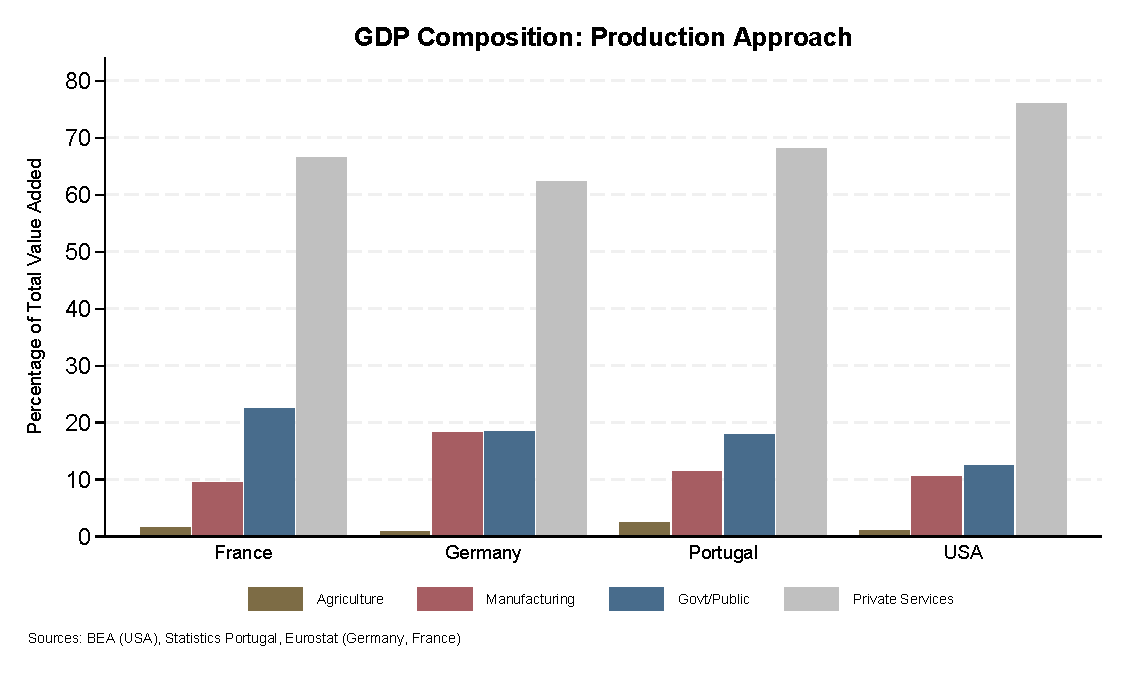
\includegraphics[width=0.9\linewidth]{figures/GDPxcountries2.pdf}
\end{center}

\end{frame}

\begin{frame}{GDP Composition}

\begin{center}
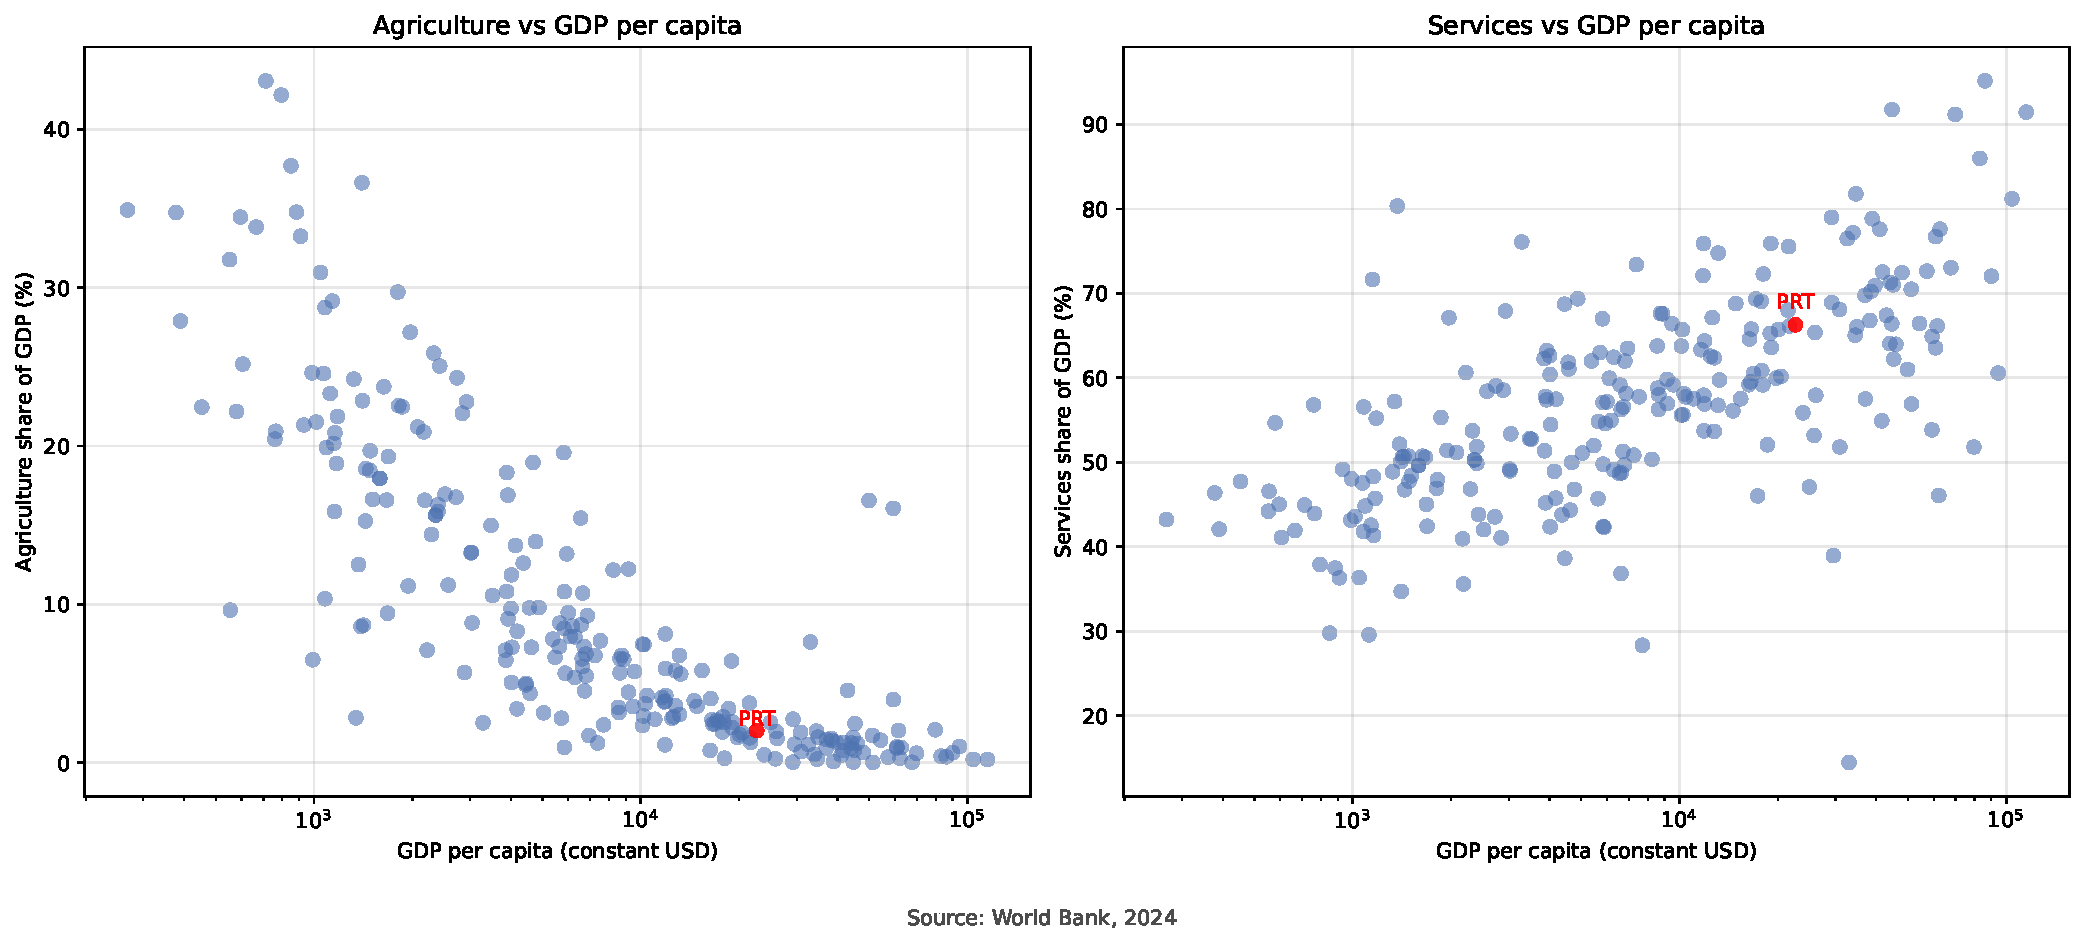
\includegraphics[width=0.9\linewidth]{figures/gdp_agri_serv.pdf}
\end{center}

\end{frame}

\begin{frame}{GDP Composition}

\begin{center}
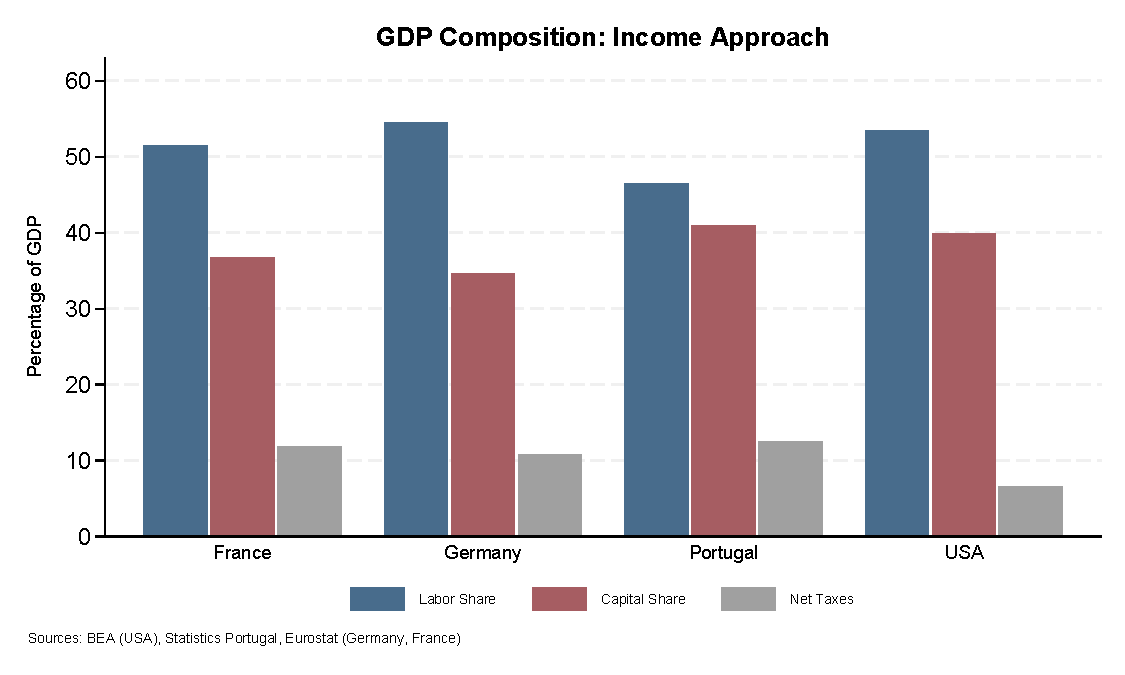
\includegraphics[width=0.9\linewidth]{figures/GDPxcountries3.pdf}
\end{center}

\end{frame}

\begin{frame}{GDP Composition}

\begin{center}
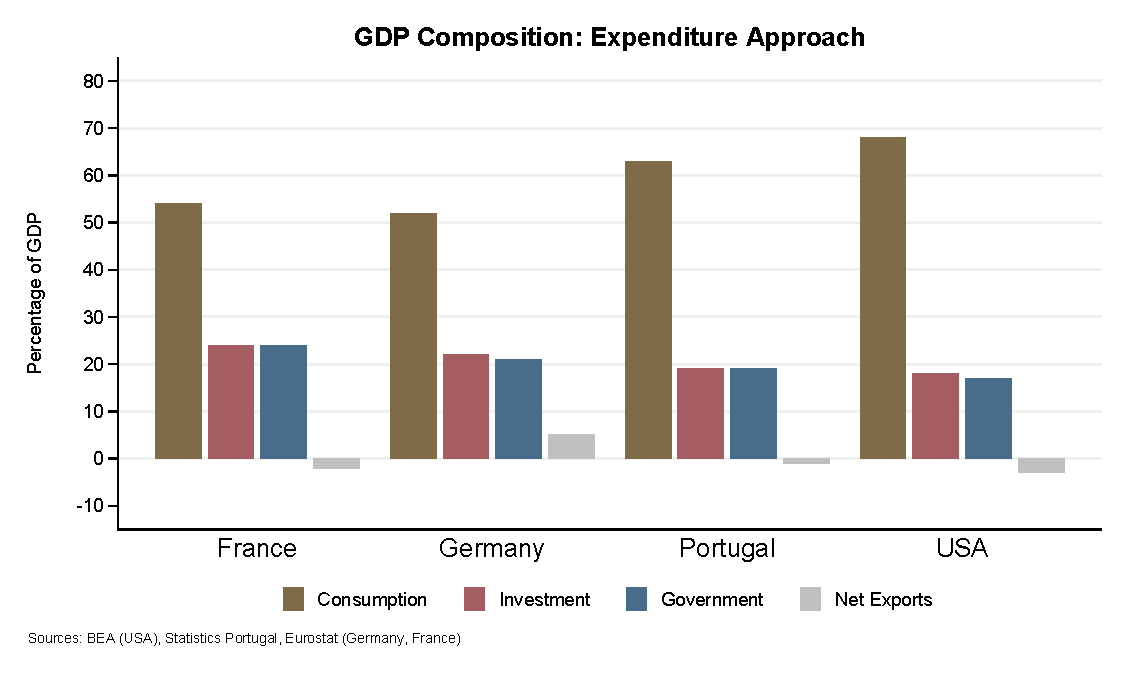
\includegraphics[width=0.9\linewidth]{figures/GDPxcountries1.pdf}
\end{center}

\end{frame}


\subsection{Making Comparisons}

\begin{frame}{Making Comparisons: Nominal vs. Real GDP}

\begin{itemize}
\item We often want to compare GDP levels not just shares:
  \begin{itemize}
  \itemvso Across \textbf{time} (e.g., 2017 vs. 2025)
    \itemvso Across \textbf{countries} (e.g., Portugal vs. Denmark)
  \end{itemize}
\itemvso But: GDP is measured in local currency (€, \$, ¥...), and prices differ across space and time.
\itemvso So the same amount of money can buy \textbf{more or less stuff}.
\end{itemize}

\end{frame}

\begin{frame}{Making Comparisons across time}{ The Country of Snackistan}

Snackistan produces only two things: burgers and yoga classes.  
Between 2023 and 2024, prices doubled, but production didn’t change.

\begin{table}
\resizebox{0.95\linewidth}{!}{%
\begin{tabular}{l r l r}
\toprule
\multicolumn{2}{c}{\textbf{2017}} & \multicolumn{2}{c}{\textbf{2018}} \\
\midrule
Burger Manufacturing (50 balls, 10 dinar each) & 500 &
Burger Manufacturing (50 balls, 20 dinar each) & 1,000 \\
Yoga Instruction (10 classes, 100 dinar each) & 1,000 &
Yoga Instruction (10 classes, 200 dinar each) & 2,000 \\
\midrule
\textbf{Total} & \textbf{1,500} & \textbf{Total} & \textbf{3,000} \\
\bottomrule
\end{tabular}
}
\end{table}


nominal GDP (in dinars) doubled, but Snackistan didn’t cook more burgers or stretch more yoga.  
\textbf{Prices doubled → Real GDP stayed the same.}
\end{frame}

\begin{frame}{The Country of Expandia}

Expandia produces only two goods: wheat and computers.  
Prices and quantities change differently between 2017 and 2018.

\begin{table}
\resizebox{0.85\linewidth}{!}{%
\begin{tabular}{l r l r}
\toprule
\multicolumn{2}{c}{\textbf{2017}} & \multicolumn{2}{c}{\textbf{2018}} \\
\midrule
Agriculture (10 tons of wheat, \$50 each) & 500 &
Agriculture (11 tons of wheat, \$60 each) & 660 \\
Manufacturing (1 computer, \$1,000 each) & 1,000 &
Manufacturing (2 computers, \$600 each) & 1,200 \\
\midrule
\textbf{Total} & \textbf{1,500} & \textbf{Total} & \textbf{1,860} \\
\bottomrule
\end{tabular}
}
\end{table}

GDP rose from \$1,500 to \$1,860 — but how much more stuff did Expandia actually produce?

\end{frame}

\begin{frame}{Making Comparisons across time}{When Prices and Quantities Both Change}

In the previous example:
\begin{itemize}
\itemvso Wheat output rose by \textbf{10\%} (10 → 11 tons)
\itemvso Computer output doubled (\textbf{+100\%})
\itemvso Prices changed differently across goods
\end{itemize}
\vspace{0.3cm}
\textbf{Question:}  
How do we measure the growth of total production when both quantities and prices move in different directions?

\begin{center}
\textit{Hint:} Use a base year to keep prices fixed!
\end{center}

\end{frame}

\begin{frame}{Making Comparisons across time}{Alternative 1: Measuring Real GDP with Base-Year Prices}

We can measure 2018 production using 2017 prices.

\begin{table}
\resizebox{0.65\linewidth}{!}{%
\begin{tabular}{l r}
\toprule
\multicolumn{2}{c}{\textbf{2018, valued at 2017 prices}} \\
\midrule
Agriculture (11 tons of wheat, \$50 each) & 550 \\
Manufacturing (2 computers, \$1,000 each) & 2,000 \\
\midrule
\textbf{Total Real GDP (2018)} & \textbf{2,550} \\
\bottomrule
\end{tabular}
}
\end{table}


\[
\text{Growth in real GDP} = \frac{2,550}{1,500} - 1 = 70\%
\]

\begin{center}
\textit{Expandia got richer in real terms — people have more stuff, not just higher prices.}
\end{center}

\end{frame}

\begin{frame}{Making Comparisons across time}{Alternative 2: Measuring Real GDP with Final-Year Prices}

We can also measure 2017 production using 2018 prices.

\begin{table}
\resizebox{0.65\linewidth}{!}{%
\begin{tabular}{l r}
\toprule
\multicolumn{2}{c}{\textbf{2017, valued at 2018 prices}} \\
\midrule
Agriculture (10 tons of wheat, \$60 each) & 600 \\
Manufacturing (1 computer, \$600 each) & 600 \\
\midrule
\textbf{Total Real GDP (2017)} & \textbf{1,200} \\
\bottomrule
\end{tabular}
}
\end{table}


\[
\text{Growth in real GDP} = \frac{1,860}{1,200} - 1 = 55\%
\]

\begin{center}
\textit{Measured at 2018 prices, growth looks smaller because computer prices fell.}
\end{center}

\end{frame}


%-----------------------------------
\begin{frame}{Making Comparisons across time}{Real GDP with Chained Prices}

\begin{itemize}
    \item The base-year and current-year price methods can give very different results. 
    \itemvso The \textbf{chained method} combines both approaches.
    \itemvso Idea:
    \begin{enumerate}
        \itemvso Start from a base year (say 2017).
        \itemvso Compute growth between consecutive years twice:
        \begin{itemize}
            \itemvso once using initial-year prices,
            \itemvso once using final-year prices.
        \end{itemize}
        \itemvso Take an average the two growth rates.
        \itemvso ``Chain'' this growth forward year by year.
    \end{enumerate}
\end{itemize}

\bigskip
\centering
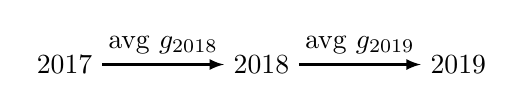
\begin{tikzpicture}[node distance=2.5cm,>=latex]
\node (a) {2017};
\node[right of=a] (b) {2018};
\node[right of=b] (c) {2019};
\draw[->, thick] (a) -- (b) node[midway, above] {avg $g_{2018}$};
\draw[->, thick] (b) -- (c) node[midway, above] {avg $g_{2019}$};
\end{tikzpicture}


\end{frame}

%-----------------------------------
\begin{frame}{Making Comparisons across time}{Real GDP with Chained Prices (Formulas)}

\[
\begin{aligned}
g_t^I &= \frac{\sum_i p_{i,t-1} q_{i,t}}{\sum_i p_{i,t-1} q_{i,t-1}} - 1 
&& \text{(growth at initial-year prices)} \\[6pt]
g_t^F &= \frac{\sum_i p_{i,t} q_{i,t}}{\sum_i p_{i,t} q_{i,t-1}} - 1 
&& \text{(growth at final-year prices)} \\[6pt]
g_t &= \sqrt{(1+g_t^I)(1+g_t^F)} - 1 
&& \text{(geometric average growth)} \\[6pt]
Y_t &= Y_{t-1}(1+g_t)
&& \text{(chain forward real GDP)}
\end{aligned}
\]

\bigskip
\begin{block}{Intuition}
The geometric average ensures a balanced measure between initial and final price weighting. 
Chaining allows comparison across many years without fixing prices from a distant base year.
\end{block}

\end{frame}

\begin{frame}{Making Comparisons across time}

\begin{center}
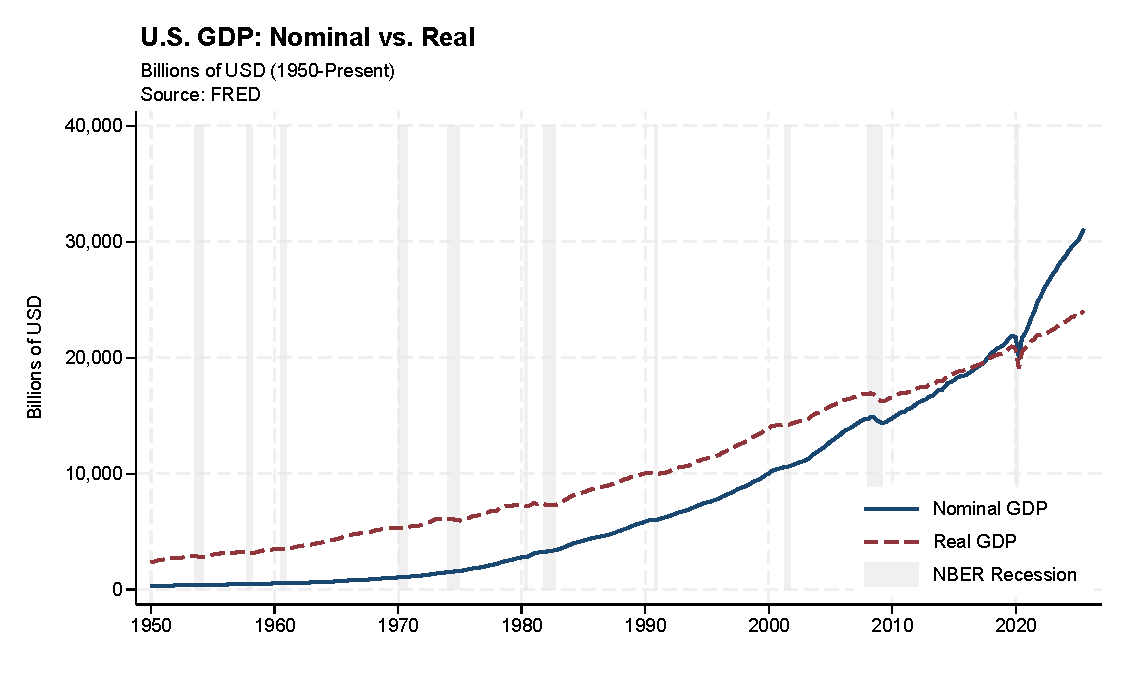
\includegraphics[width=0.9\linewidth]{figures/US_GDP_nominal_vs_real.pdf}
\end{center}

\end{frame}
%-----------------------------------

\subsection{Comparison Across Countries and PPP}

%-----------------------------------
\begin{frame}{Comparing GDP Across Countries}

\begin{itemize}
    \item Suppose we want to compare GDP between the US and Mexico in 2018:
    \begin{table}
    \resizebox{0.8\linewidth}{!}{%
    \begin{tabular}{l r l r}
    \toprule
    Country & GDP & Population & GDP per capita \\
    \midrule
    United States & 20.5 trillion \$ & 327 million & 62,700 \$ per person \\
    Mexico & 23.5 trillion pesos & 127 million & 185,000 pesos per person \\
    \bottomrule
    \end{tabular}
    }
    \end{table}

    \itemvso Can we say Mexicans produced more output per person than U.S residents? Not yet — the currencies are different!
\end{itemize}

\end{frame}


%-----------------------------------
\begin{frame}{Using Market Exchange Rates}

\begin{itemize}
    \item One way to compare GDP is using the market exchange rate (MER):
    \[
        \text{GDP in USD} = \text{GDP in local currency} \times \text{Exchange rate (USD/local)}
    \]
    \itemvso For Mexico in 2018: $23.5 \text{trillion pesos} \times 0.051 USD/peso \simeq 1.2  \text{trillion USD}$.
    \itemvso Converted per capita: $1.2  \text{trillion USD} \div 127 \text{million people} \simeq 9,500 \text{USD per person}$.
    \itemvso Problems with market rates:
    \begin{itemize}
        \item Exchange rates fluctuate daily and may not reflect domestic prices.
        \itemvso Non-traded goods (housing, services) are cheaper in developing countries, so MER underestimates real living standards.
    \end{itemize}
\end{itemize}

\begin{block}{Takeaway}
Market exchange rates give a currency-based comparison, but do not capture what people can actually buy.
\end{block}

\end{frame}



%-----------------------------------
\begin{frame}{Using Purchasing Power Parity (PPP)}

\begin{itemize}
    \item PPP adjusts for differences in the cost of living:
    \[
        \text{GDP in Foreign Country at PPP} = \sum_i p_i^{\text{US}} \cdot q_i^{\text{foreign}}
    \]
    where \(p_i^{\text{US}}\) is the US price of good \(i\), \(q_i^{\text{foreign}}\) is the foreign quantity.
    \itemvso For Mexico, PPP-adjusted per capita GDP $\approx$ 18,000 USD, almost double the market-rate conversion.
\end{itemize}

\begin{block}{Intuition}
PPP measures what residents could actually buy if they lived in the US. Market exchange rates only tell you the currency value, not purchasing power.
\end{block}

\end{frame}

%-----------------------------------
\begin{frame}{PPP Exchange Rates and the Big Mac Index}

\begin{itemize}
    \item The PPP exchange rate is the rate that makes GDP at market exchange and GDP at PPP coincide:
    \[
        \text{PPP exchange rate} = \frac{\text{GDP in dollars at PPP}}{\text{GDP in local currency}}
    \]
    \item Fun illustration: \textbf{The Big Mac Index}.
    \begin{itemize}
        \item Compare the price of a Big Mac in the US and abroad.
        \item Example: if a Big Mac costs \$5 in the US and 50 pesos in Mexico, the implied PPP exchange rate is 1 USD = 10 pesos.
        \item A playful way to see which currencies are “overvalued” or “undervalued.”
    \end{itemize}
\end{itemize}

\end{frame}

\begin{frame}{Comparing GDP Across Countries}
\begin{center}
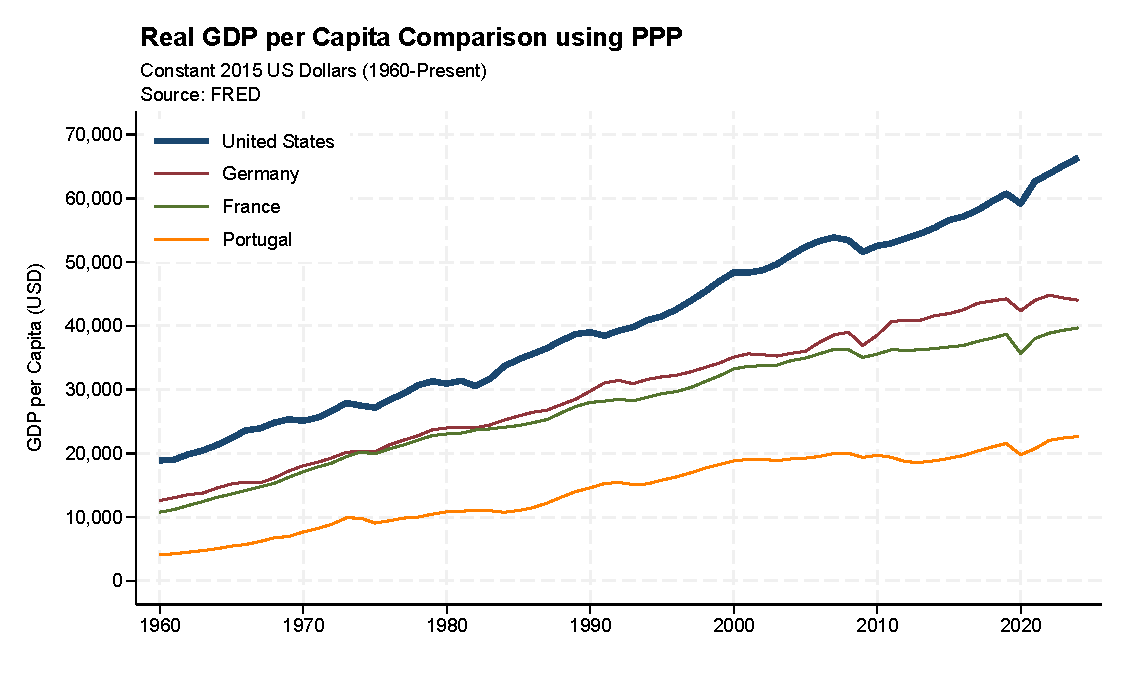
\includegraphics[width=0.9\linewidth]{figures/GDP_Per_Capita_Comparison.pdf}
\end{center}
\end{frame}

\begin{frame}{Comparing GDP Across Countries}
\begin{center}
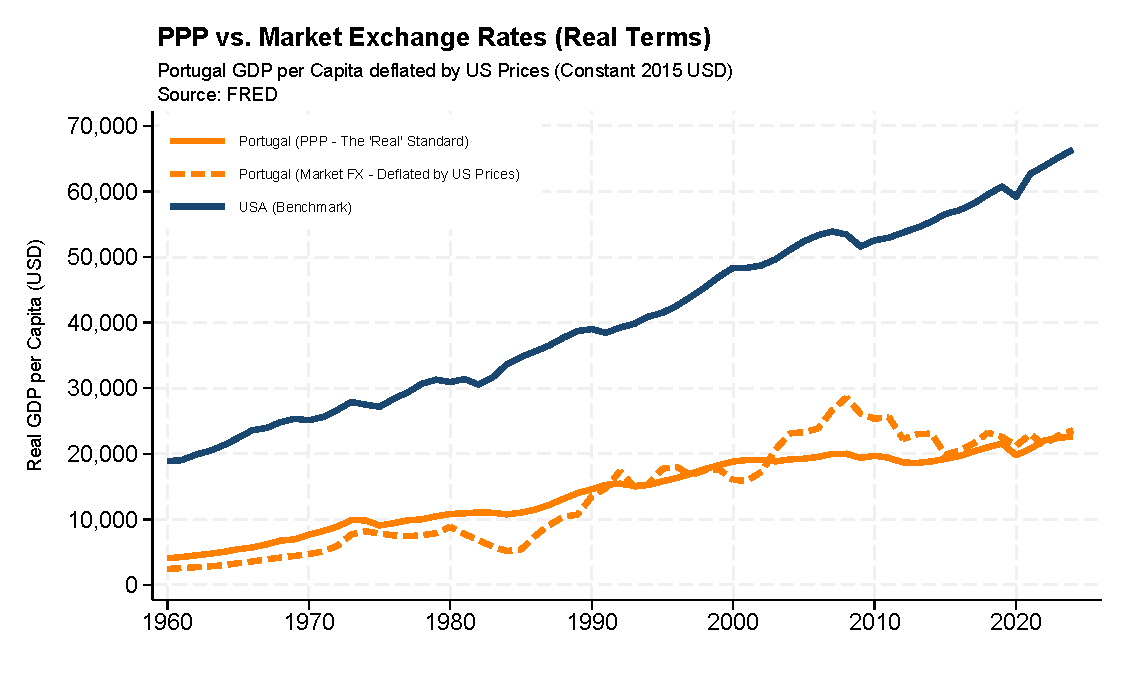
\includegraphics[width=0.9\linewidth]{figures/GDP_Per_Capita_PPP_vs_Mkt.pdf}
\end{center}
\end{frame}





\section{Beyond GDP}

\begin{frame}{Beyond GDP — Measuring Development}

\begin{itemize}
    \item GDP is a powerful indicator of economic activity, but it does not capture everything we care about.
    \itemvso Economic \textbf{development} involves more than production and income:
    \begin{itemize}
        \item Health and life expectancy
        \item Education and literacy
        \item Access to opportunities and basic services
    \end{itemize}
    \itemvso Now, we discuss alternative ways to measure well-being and living standards.
\end{itemize}

\end{frame}

\subsection{The Human Development Index}
\begin{frame}{The Human Development Index (HDI)}

\begin{itemize}
    \item Created by the United Nations Development Programme (UNDP).
    \itemvso Combines three key dimensions of human well-being:
    \begin{enumerate}
        \itemvso \textbf{Health:} measured by life expectancy at birth.
        \itemvso \textbf{Education:} measured by average and expected years of schooling.
        \itemvso \textbf{Income:} measured by GNI per capita (PPP adjusted).
    \end{enumerate}
    \itemvso Each dimension is normalized between 0 and 1, and the HDI is their geometric mean:
    \[
    \text{HDI} = (I_{\text{health}} \cdot I_{\text{education}} \cdot I_{\text{income}})^{1/3}
    \]
\end{itemize}


\end{frame}

\begin{frame}{The Human Development Index (HDI)}

\begin{figure}
    \centering
    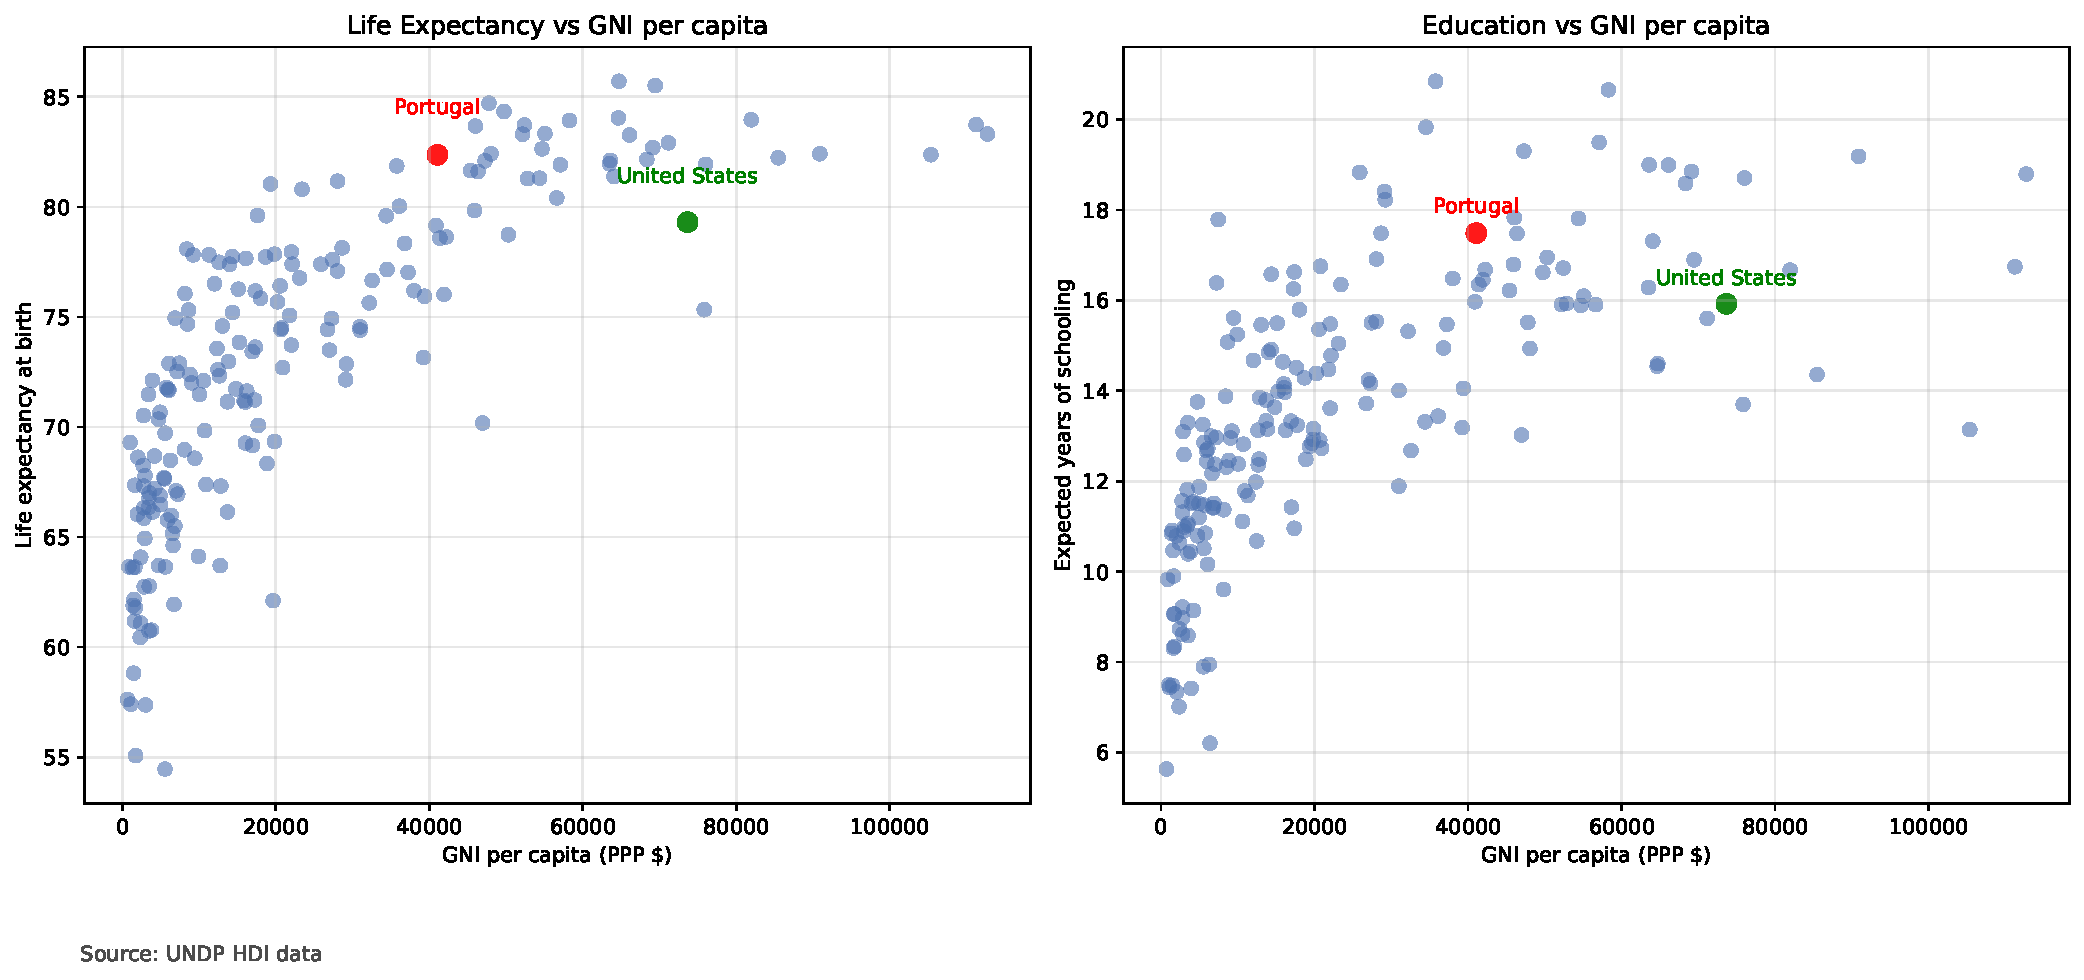
\includegraphics[width=0.9\linewidth]{figures/gni_life_edu_us_pt.pdf}
\end{figure}

\end{frame}

\begin{frame}{The Human Development Index (HDI)}

\begin{figure}
    \centering
    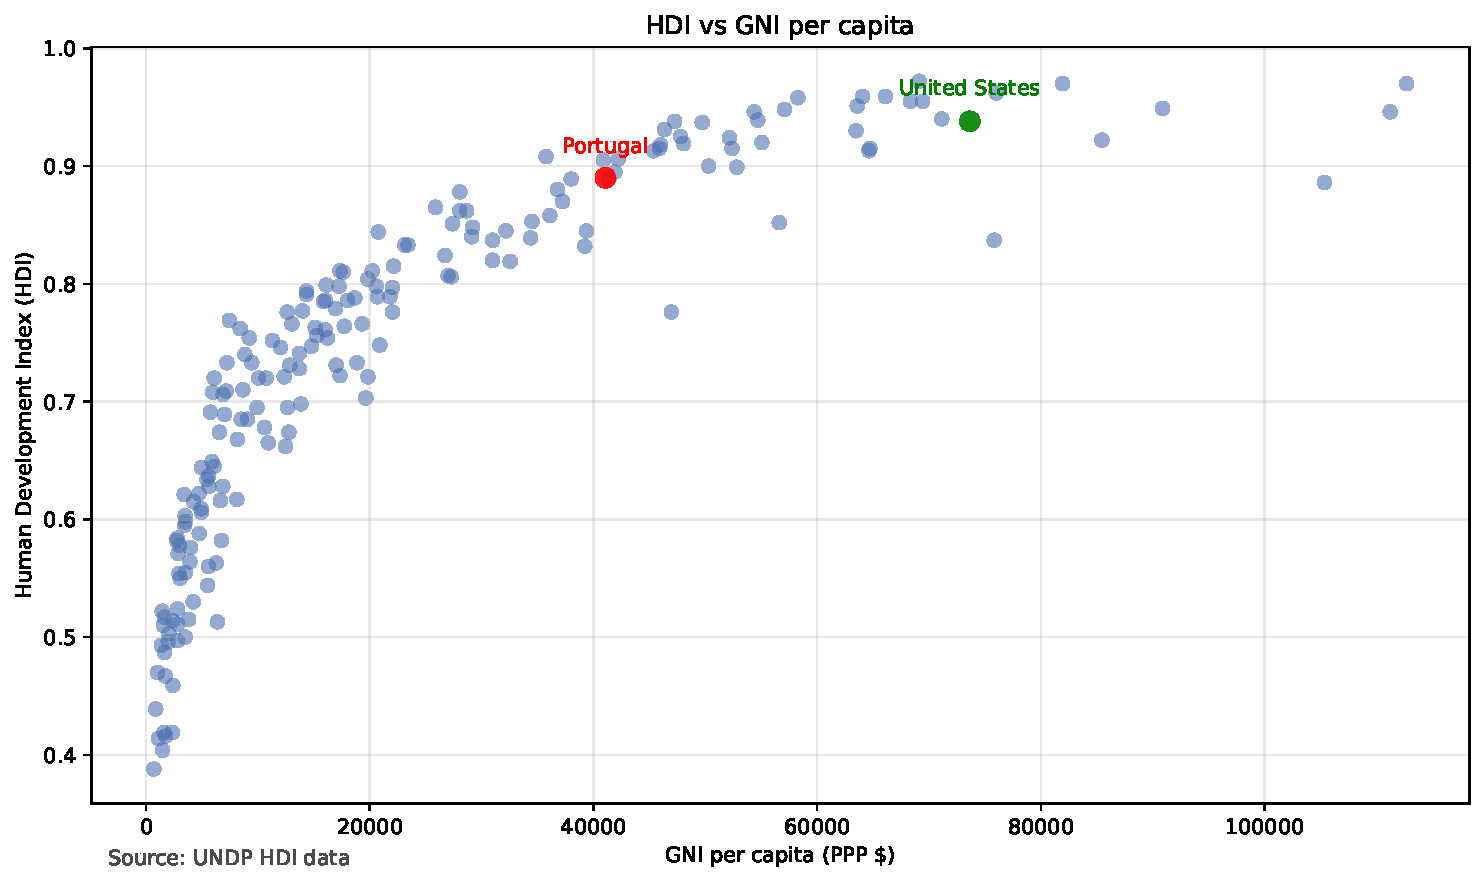
\includegraphics[width=0.9\linewidth]{figures/gni_hdi_us_pt.pdf}
\end{figure}

\end{frame}


\begin{frame}{The Human Development Index (HDI)}

\begin{itemize}

\item One unsatisfying aspect of the HDI is that the scaling and weighting of the various factors is arbitrary.
\begin{itemize}
\itemvso What exactly is the HDI measuring?
\itemvso Why convert variables into indices?
\itemvso Why equal weights on the three factors?
\end{itemize} 
\end{itemize}
\end{frame}

\subsection{Jones \& Klenow (2016)}

\begin{frame}{Beyond GDP: Jones \& Klenow (2016)}
\begin{itemize}
  \item Jones \& Klenow propose a \textbf{welfare measure} similar in spirit to the HDI but grounded in \textbf{utility theory}.
  \itemvso They aim to include aspects of life that GDP misses, focusing on:
  \begin{itemize}
    \itemvso \textbf{Consumption} – what people actually enjoy, not just produce,
    \itemvso \textbf{Leisure and nonmarket production} – time spent outside work counts too,
    \itemvso \textbf{Life expectancy} – how long people live,
    \itemvso \textbf{Inequality} – differences in consumption across people.
  \end{itemize}
\end{itemize}
\end{frame}

% -------------------------
\begin{frame}{Individual Utility in Jones \& Klenow (2016)}
\begin{itemize}
  \item Each individual derives utility from:
  \begin{itemize}
    \itemvso \textbf{Consumption} (\(c\)): goods and services enjoyed,
    \itemvso \textbf{Leisure} (\(\ell\)): time not spent working,
    \itemvso \textbf{Life status} (\(a\)): alive (\(a=1\)) or dead (\(a=0\)).
  \end{itemize}

  \itemvso Utility is modeled as:
  \[
  u(c,\ell,a)
  =
  \Big(
  \bar{u}
  + \frac{c^{1-\sigma}}{1-\sigma}
  - \theta(1-\ell)^2
  \Big){a}
  \]

  \item Key parameters:
  \begin{itemize}
    \item \(\bar{u}\): baseline utility from being alive,
    \item \(\sigma\): risk aversion (how much people dislike inequality and uncertainty),
    \item \(\theta\): importance of leisure.
  \end{itemize}

  \itemvso Being dead gives utility \(0\) by convention.
\end{itemize}
\end{frame}
% -------------------------


% -------------------------
\begin{frame}{The Experiment: Comparing Portugal to the U.S.}
\begin{itemize}
  \item Imagine a person — let’s call him \textbf{Pat the Alien} — who must choose where to live for a year:
  \begin{enumerate}
    \itemvsoo As a random resident in \textbf{Portugal},
    \itemvso As a random resident in the \textbf{United States}
  \end{enumerate}

  \itemvso When choosing, Pat the Alien does not know which individual they will be:
  \begin{itemize}
    \itemvsoo a banker in Chiado or a waiter in Alfama,
    \itemvso a surfer in Ericeira or a stressed consultant in Lisbon,
    \itemvso alive or dead.
  \end{itemize}

  \itemvso In other words, Pat chooses under \textbf{uncertainty}.
  \itemvso We need a way to quantify which country would be preferred: expected utility.
\end{itemize}
\end{frame}

% -------------------------
\begin{frame}{Expected Utility Across Individuals}
\begin{itemize}
  \item Pat the Alien knows the possible outcomes in each country (consumption, leisure, life expectancy) but not which one he will experience.
  \itemvso Examples:
  \begin{itemize}
    \item Ana or João in Portugal,
    \item Mike or Diane in the U.S.
  \end{itemize}

  \itemvso Pat will prefer the country that gives the \textbf{highest expected utility}:
  \[
  U = \mathbb{E}\Big[
  (\bar{u} + \frac{c^{1-\sigma}}{1-\sigma} - \theta (1-\ell)^2) a
  \Big]
  = \frac{1}{N} \sum_{i=1}^N (\bar{u} + \frac{c_i^{1-\sigma}}{1-\sigma} - \theta (1-\ell_i)^2) a_i
  \]

  \item This is a simple application of \textbf{expected utility theory}: uncertain outcomes are evaluated by weighting each possible utility by its probability.
\end{itemize}
\end{frame}


\begin{frame}{The Role of Risk Aversion (\(\sigma\)) in Utility}
\begin{itemize}
  \item In expected utility theory, people's attitudes toward risk are captured by the \textbf{concavity of the utility function}.
  \itemvso We use concavity in models to capture the idea that \textbf{most people dislike uncertainty} and therefore Pat the alien would prefer countries with lower inequality.
  \itemvso Mathematically, holding leisure (\(\ell\)) and life status (\(a\)) constant, utility is a function of consumption \(c\):
  \[
  u(c) = \frac{c^{1-\sigma}}{1-\sigma}
  \]
\end{itemize}
\end{frame}


% -------------------------
\begin{frame}{Pat the Alien and Risky Choices}
\begin{itemize}
  \item Suppose there are two people in Portugal: one rich (\(c_{\text{rich}}\)) and one poor (\(c_{\text{poor}}\)).
  \itemvso Pat the Alien could end up in either situation with probability \(1/2\).
  \itemvso Pat is \textbf{risk averse} if he prefers a the average consumption over facing uncertainty:
  \[
  u\Big(\frac{c_{\text{rich}} + c_{\text{poor}}}{2}\Big) 
  > \frac{u(c_{\text{rich}}) + u(c_{\text{poor}})}{2}
  \]
\end{itemize}
\end{frame}

% -------------------------
\begin{frame}{Concavity and Marginal Utility}
\begin{itemize}
  \item The concavity of the utility function is controlled by \(\sigma\):
  \begin{itemize}
    \itemvso High \(\sigma\) → very concave: Pat strongly dislikes inequality and risk.
    \itemvso Low \(\sigma\) → almost linear: Pat is less sensitive to differences across states.
  \end{itemize}

\end{itemize}
\end{frame}

% -------------------------
\begin{frame}{How Do We Choose \(\sigma\) in Practice?}
\begin{itemize}
  \item People have different attitudes towards risk → we pick \(\sigma\) to represent an average individual: Pat.
  \itemvso Empirical methods:
  \begin{itemize}
    \itemvso Investment choices: how much risk vs. average return are people willing to bear?
    \itemvso Insurance decisions: willingness to pay for smoothing consumption across uncertain states.
  \end{itemize}
  \itemvso Estimates range from \(\sigma \approx 1\) (mildly risk averse) to \(\sigma \approx 10\) (very risk averse).
  \itemvso When choosing where Pat want to live, \(\sigma\) determines how much Pat cares about inequality:
  \begin{itemize}
    \itemvso High \(\sigma\) → unequal country looks risky: egalitarian countries become more attractive to Pat
    \itemvso Low \(\sigma\) → countries with higher expected income are more attractive
  \end{itemize}
\end{itemize}
\end{frame}


\begin{frame}{The Value of Life Expectancy (\(\bar{u}\))}
\begin{itemize}
  \item Pat the Alien does not know is he will be dead or alive.
  \itemvso Suppose Pat's age is randomly drawn from 0 to 100:
  \begin{itemize}
    \itemvso If his age exceeds life expectancy in the country, he is dead → utility = 0
    \itemvso If he is alive → utility = \(\bar{u} + \frac{c^{1-\sigma}}{1-\sigma} - \theta(1-\ell)^2\)
  \end{itemize}
  \itemvso Everyone alive gets the baseline utility \(\bar{u}\) in addition to consumption and leisure utility.
\end{itemize}
\end{frame}

\begin{frame}{The Value of Leisure and Non-Market Production (\(\theta\))}

\begin{itemize}
  \item People can spend their time in different ways:
  \begin{itemize}
    \item Market work → counted in GDP
    \item Non-market activities → not counted in GDP (cleaning, cooking, childcare)
    \item Pure leisure → reading, watching TV, surfing, etc.
  \end{itemize}

  \itemvso In our utility function, \( \ell \) is the fraction of time spent on non-market and leisure activities.

  \itemvso The parameter \(\theta\) captures how much people value non-market activities (or dislike market work).

  \itemvso How can we measure \(\theta\)?
  \begin{itemize}
    \item Look at trade-offs people make between consumption and free time
    \item Use choices like labor force participation, retirement age, weekly work hours, holidays
    \item Higher \(\theta\) → people work less, enjoy more leisure and non-market activities
  \end{itemize}

  \itemvso By matching observed time allocation between market and non-market activities, we can estimate \(\theta\).
\end{itemize}
\end{frame}


\begin{frame}{Comparing Living Standards Across Countries: Intuition}

\begin{itemize}
  \item We want a metric that tells us \textbf{how much better or worse life is in Portugal vs. the U.S.} in an intuitive way.
  
  \itemvso Expected utility is great for theory, but \emph{utiles are abstract}. Students, policymakers, and citizens care about consumption, leisure, and life expectancy in \textbf{familiar units}.
  
  \itemvso Enter \(\lambda^{PT}\): a \textbf{consumption scaling factor} for the U.S. that makes a random resident just as happy as in Portugal:
  \[
   \dfrac{1}{N}\sum_{i=1}^n u(\lambda^{PT} c_i^{US}, \ell_i^{US}, a_i^{US}) = U^{PT}
  \]
  \vspace{-1.5em}
  \itemvso Intuition:
  \begin{itemize}
    \item \(\lambda^{PT} > 1\): You need more U.S. consumption to match Portugal → Portugal is ``better" in welfare terms.
    \itemvso \(\lambda^{PT} < 1\): Portuguese residents need more consumption to match the U.S. → U.S. is ``better".
  \end{itemize}
\end{itemize}

\end{frame}

\begin{frame}{Comparing Living Standards Across Countries: Computation}

\begin{itemize}
  \item Step 1: Compute the expected utility in Portugal:
  \[
  U^{PT} = \frac{1}{N} \sum_{i=1}^{N} u(c_i^{PT}, \ell_i^{PT}, a_i^{PT})
  \]
  \vspace{-1.5em}
  \item Step 2: Solve for \(\lambda^{PT}\) in:
  \[
  U^{PT} = \frac{1}{N} \sum_{i=1}^{N} u(\lambda^{PT} c_i^{US}, \ell_i^{US}, a_i^{US})
  \]
  \vspace{-1.5em}
  \item Step 3: Interpret \(\lambda\):
  \begin{itemize}
    \item \(\lambda^{PT} = 1.2\) → Portugal provides the same welfare as the U.S. with 20\% higher consumption.  
    \item \(\lambda^{PT} = 0.9\) → Portugal provides the same welfare as the U.S. with 10\% lower consumption.
  \end{itemize}

  \itemvso Example: Suppose the expected utility in Portugal is \(10.5\) utiles and in the U.S. it is \(11\) utiles. Solving for \(\lambda^{PT}\) gives \(\lambda = 0.95\) → Portugal is slightly worse off in equivalent U.S. consumption terms.
  
\end{itemize}

\end{frame}

\begin{frame}{Results: Welfare (\(\lambda\)) vs. GDP per Capita}


\begin{figure}
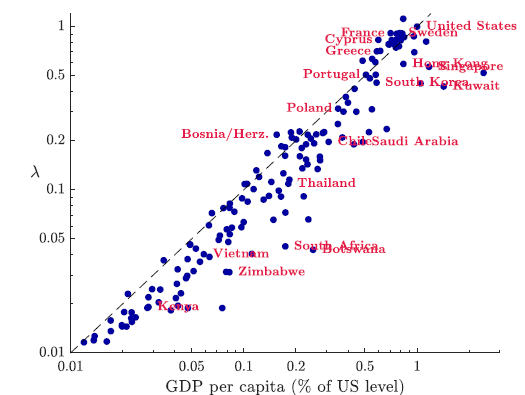
\includegraphics[width=0.7\textwidth]{figures/scatter_lambda_gdp.png}
\caption{Relative GDP and welfare. Source: Jones and Klenow (2016).}
\end{figure}



\end{frame}

\begin{frame}{HDI vs. Jones \& Klenow (2016)}

\begin{itemize}
  \item \textbf{HDI:} 
  \begin{itemize}
    \itemvso Simple composite index of life expectancy, education, and income
    \itemvso Assumptions are mostly implicit or not clearly listed
    \itemvso No clear rationale for how components are weighted
    \itemvso Provides a single number, but it is hard to know what it really means or how it was constructed
  \end{itemize}

  \itemvso \textbf{Jones \& Klenow (2016):}
  \begin{itemize}
    \itemvso Grounded in utility theory—parameters explicitly defined
    \itemvso Incorporates consumption, leisure, life expectancy, and inequality
    \itemvso Assumptions are explicit: if you disagree, you can modify the model
    \itemvso Provides a number (\(\lambda\)) that is interpretable and based on the model structure
  \end{itemize}
\end{itemize}

\end{frame}


\begin{frame}{Takeaways for Economic Research}

\begin{itemize}
  \item Models are simplifications of reality, just like a map is a simplification of geography
  \itemvso Explicit assumptions make progress possible:
  \begin{itemize}
    \itemvso We know what drives results
    \itemvso We can test alternative assumptions
    \itemvso We can propose improvements and extensions
  \end{itemize}
  
  \itemvso If you see a missing feature in current research:
  \begin{itemize}
    \itemvso Try writing a model that incorporates it
    \itemvso Analyze whether it makes a difference
    \itemvso This is the essence of research in economics: theory + data + clear assumptions
  \end{itemize}
  
\end{itemize}

\end{frame}


%\section{Population Aging}
%
%\begin{frame}{Aging: the Central Challenges of Our Time}
%
%\begin{itemize}
%\item The defining economic force of the 21st century is \textbf{population aging}.
%\itemvso Advanced economies are experiencing a rapid increase in the share of older individuals,
%  combined with a stagnating or shrinking working-age population.
%\itemvso The economic consequences can be profound:
%\begin{itemize}
%    \itemvso Economic growth: fewer workers, lower potential output growth.
%    \itemvso Public finances: pressure on pensions, healthcare, and long-term care systems.
%    \itemvso Inequality: generational redistribution within and across generations
%\end{itemize}
%
%\itemvso Understanding aging is therefore essential for analyzing growth, fiscal policy,
%and long-run sustainability and analyzing GDP statistics allows us to get a sense of what is coming
%\end{itemize}
%
%\end{frame}
%
%\begin{frame}{Aging Across Economies}{ Old Age Dependency}
%\centering
%\includegraphics[width=0.9\linewidth]{figures/aging_old_dependency_US_Europe_Japan.pdf}
%\end{frame}
%
%
%\begin{frame}{Aging Across Economies}{ Government Expenses: Young and Old }
%\centering
%\includegraphics[width=1\linewidth]{figures/expenditure_trends.pdf}
%\end{frame}
%
%\begin{frame}{Aging Across Economies}{ Government Expenses: Young and Old }
%\centering
%\includegraphics[width=1.0\linewidth]{figures/US_expenditure_WIDE.pdf}
%\end{frame}

\end{document}
